%%%  default
\documentclass[10pt, compress]{beamer}


\usetheme{mnuig}
\usepackage{tikz}
\usepackage{booktabs}
%\usepackage{cite}
\bibliographystyle{apalike}

%\usepackage[scale=2]{ccicons}

%\usemintedstyle{trac}
\usepackage{grffile} %for underscores in file names

\title{Lab Meeting}
\subtitle{}
\date{\footnotesize{\today}}
\author{\\ \\ \\ \\Nick Waters}
\institute{Department of Microbiology\\
School of Natural Sciences\\
National University of Ireland Galway}

%%%%% %%%%% %%%%% %%% %%%%  for pretty headers with pictures
\addtobeamertemplate{frametitle}{}{%
\begin{tikzpicture}[remember picture,overlay]
\node[anchor=north east,yshift=2pt] at (current page.north east) {
\includegraphics[height=0.8cm]{../stock_logos/nuig_rounded.png}  \hspace*{.05cm} 
\includegraphics[height=.794cm, trim= 0cm 0.0cm 0.0cm 0cm]{../stock_logos/jhi_rounded.png}};
\end{tikzpicture}}




\begin{document}

%\maketitle
\section{Short Ready Assembly}

\begin{frame}[fragile]
  \frametitle{Problems}
  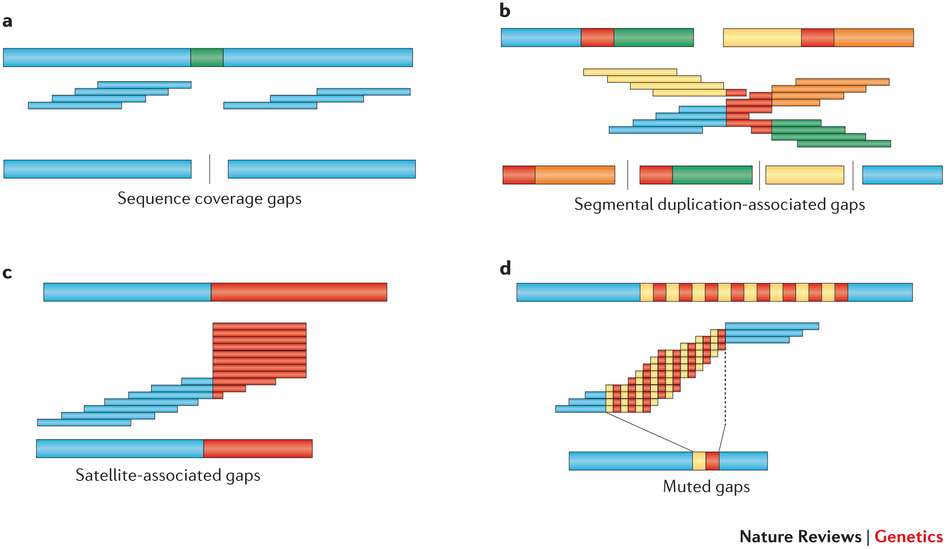
\includegraphics[width=\textwidth]{/home/nicholas/GitHub/FB/Ecoli_comparative_genomics/doc/presentations/MyNUIG(mnuigtheme)/frequentFigs/nature.jpg}\\\tiny {Source\cite{Chaisson2015}}
\end{frame}


\begin{frame}[fragile]
  \frametitle{de Bruijn Graphs and Eulerian Paths}
  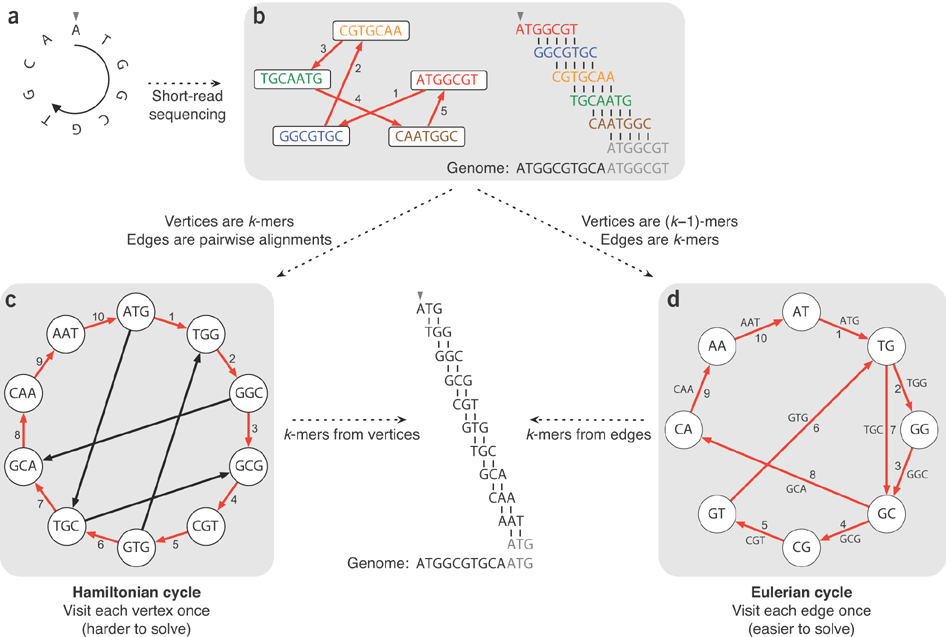
\includegraphics[width=\textwidth]{/home/nicholas/GitHub/FB/Ecoli_comparative_genomics/doc/presentations/MyNUIG(mnuigtheme)/frequentFigs/Compeau2011.png}\\\tiny {Source\cite{Compeau2011}}
\end{frame}


\begin{frame}[fragile]
  \frametitle{Eulerian Paths with Repeats}
  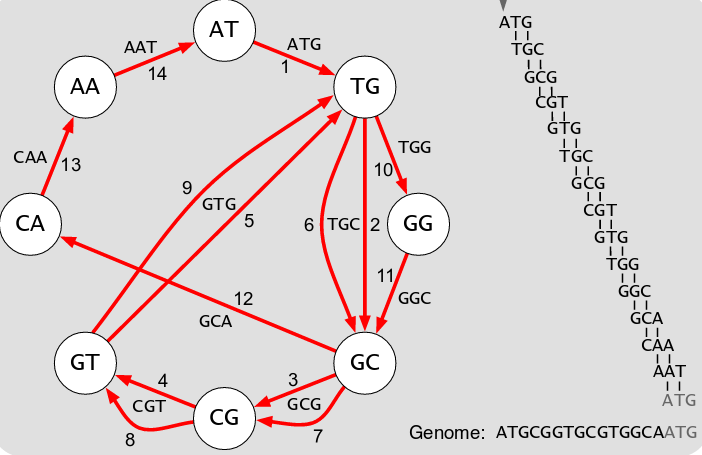
\includegraphics[width=\textwidth]{/home/nicholas/GitHub/FB/Ecoli_comparative_genomics/doc/presentations/MyNUIG(mnuigtheme)/frequentFigs/Compeau2_2011.png}\\\tiny {Source\cite{Compeau2011}}
\end{frame}



\begin{frame}[fragile]
  \frametitle{Improving Illumina Short Read Assembly}
\begin{enumerate}
\item Within a taxanomic group, GC content is largely conserved.
\item Within a taxonomic group, genome size is largely conserved.
\item Bacterial genomes are dense.
\item Nucleotide order is not random.
\end{enumerate}

\end{frame}
\begin{frame}[fragile]
  \frametitle{Possible Solution}
  \begin{figure}
% see

\definecolor{cb3b3b3}{RGB}{179,179,179}
\definecolor{cffaaaa}{RGB}{255,170,170}
\definecolor{cdeaa87}{RGB}{222,170,135}
\definecolor{cff9955}{RGB}{255,153,85}


\begin{tikzpicture}[y=0.80pt, x=0.80pt, yscale=-1.00000, xscale=1.000000, inner sep=0pt, outer sep=0pt]
\path[draw=black,fill=cb3b3b3,miter limit=4.00,draw opacity=0.000,line
  width=0.137pt,rounded corners=0.0000cm] (98.0545,56.3976) rectangle
  (304.3740,66.3267);
\path[draw=black,fill=cffaaaa,miter limit=4.00,draw opacity=0.000,line
  width=0.061pt,rounded corners=0.0000cm] (92.8397,84.3501) rectangle
  (132.8746,94.3743);
\path[draw=black,fill=cffaaaa,miter limit=4.00,draw opacity=0.000,line
  width=0.061pt,rounded corners=0.0000cm] (152.8397,102.3501) rectangle
  (192.8746,112.3743);
\path[draw=black,fill=cffaaaa,miter limit=4.00,draw opacity=0.000,line
  width=0.061pt,rounded corners=0.0000cm] (102.8397,102.3501) rectangle
  (142.8746,112.3743);
\path[draw=black,fill=cffaaaa,miter limit=4.00,draw opacity=0.000,line
  width=0.061pt,rounded corners=0.0000cm] (122.8397,122.3501) rectangle
  (162.8746,132.3743);
\path[draw=black,fill=cffaaaa,miter limit=4.00,draw opacity=0.000,line
  width=0.061pt,rounded corners=0.0000cm] (139.2682,84.4929) rectangle
  (179.3032,94.5172);
\path[draw=black,fill=cffaaaa,miter limit=4.00,draw opacity=0.000,line
  width=0.061pt,rounded corners=0.0000cm] (228.5539,87.3501) rectangle
  (268.5889,97.3743);
\path[draw=black,fill=cffaaaa,miter limit=4.00,draw opacity=0.000,line
  width=0.061pt,rounded corners=0.0000cm] (246.8397,106.3501) rectangle
  (286.8746,116.3743);
\path[draw=black,fill=cffaaaa,miter limit=4.00,draw opacity=0.000,line
  width=0.061pt,rounded corners=0.0000cm] (272.8397,122.3501) rectangle
  (312.8746,132.3743);
\path[draw=black,fill=cffaaaa,miter limit=4.00,draw opacity=0.000,line
  width=0.061pt,rounded corners=0.0000cm] (262.8397,142.3501) rectangle
  (302.8746,152.3743);
\path[draw=black,fill=cffaaaa,miter limit=4.00,draw opacity=0.000,line
  width=0.061pt,rounded corners=0.0000cm] (226.8397,124.3501) rectangle
  (266.8746,134.3743);
\path[draw=black,fill=cdeaa87,miter limit=4.00,draw opacity=0.000,line
  width=0.061pt,rounded corners=0.0000cm] (187.8397,145.9215) rectangle
  (227.8746,155.9457);
\path[draw=black,fill=cffaaaa,miter limit=4.00,draw opacity=0.000,line
  width=0.061pt,rounded corners=0.0000cm] (252.8397,72.3501) rectangle
  (292.8746,82.3743);
\path[draw=black,fill=cff9955,miter limit=4.00,draw opacity=0.000,line
  width=0.069pt,rounded corners=0.0000cm] (182.8517,32.3551) rectangle
  (234.2911,42.3693);

\end{tikzpicture}

\caption{Bridge Reconstruction. Pink fragments are reads.  Grey shows the gene of interest with interupted coverage. Orange fragemnt is a pseudoread generated from this situation under the hypothesis that the beige fragment exists but is underrepresented: that is, the bridge is there, but needing repair}
\label{fig:bridge_rec}
\end{figure}
\end{frame}

\begin{frame}[fragile]
  \frametitle{Initial Data}
  \includegraphics[width=\textwidth]{~/GitHub/FB/Ecoli_comparative_genomics/doc/notebook/figures/pca_pseudoread_assembly.pdf}
\end{frame}


\begin{frame}
%\addbibresource{myreferences.bib}
\bibliography{/home/nicholas/GitHub/FB/library}
\end{frame}

\begin{frame}{Acknowledgements}
  \begin{columns}[onlytextwidth]
    \column{0.5\textwidth}
    \includegraphics[height=1cm]{../stock_logos/NUI_Galway_BrandMark_A_K.eps}\\
     NUIG Microbiology
      \begin{itemize}
        \item Dr. Fiona Brennan
        \item Dr. Florence Abram
        \item Matthias Waibel
      \end{itemize}
      NUIG Maths
      \begin{itemize}
        \item Pilib
      \end{itemize}

    \column{0.5\textwidth}
    
\includegraphics[height=1cm]{../stock_logos/trimmed_jhi.png}\\
      James Hutton Institute
      \begin{itemize}
        \item Leighton Pritchard
      \end{itemize}
  \end{columns}
\end{frame}



\plain{}{Questions?}

\end{document}
